\documentclass[10pt,letterpaper]{article}
\usepackage[utf8]{inputenc}
\usepackage{amsmath}
\usepackage{amsfonts}
\usepackage{amssymb}
\usepackage{graphicx}

\author{Brock Ellefson}
\title{ANTY101 Lab 2}
\begin{document}
\maketitle
\newpage


%%%%%%%%%%%%%%%%%%%%%%%%%%%%%%%%%%%%%%%%%%%%%%%%%%%%%%%%%%%%%


\begin{figure}[!tbp]
	\centering
		\begin{minipage}[b]{0.4\textwidth}
			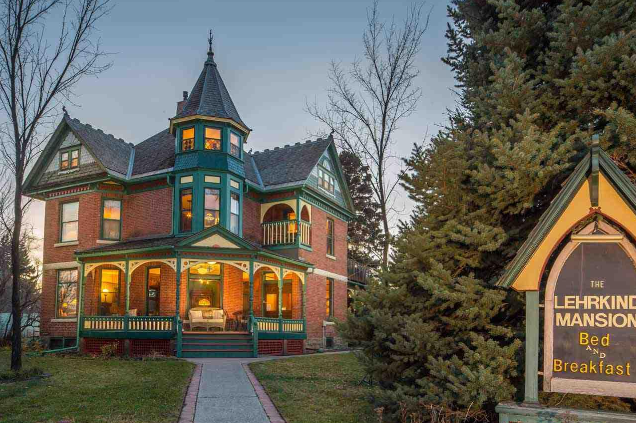
\includegraphics[width=\textwidth]{house1pic1.png}
    		\caption{719 N Wallace Avenue}
  		\end{minipage}
  \hfill
  		\begin{minipage}[b]{0.4\textwidth}
    		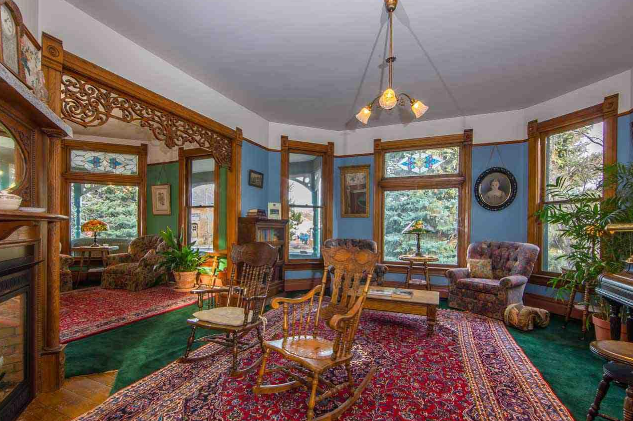
\includegraphics[width=\textwidth]{house1pic2.png}
    		\caption{719 N Wallace Avenue}
  		\end{minipage}
\end{figure}

	
The Lehrkind Mansion Bed and Breakfast is an iconic Queen Anne style building of Bozeman that was constructed in 1897. The exterior is made mainly of brick. However there is green wood trim outlining the house. 3 floors, 11 bedrooms. There is also a separate guest house on the tail end of the BnB, complete with a full bathroom and 3 bedrooms, totaling to 4,626 square feet. The driveway is paved with fine gravel. The entrance has a beautiful open porch 
%%%%%%%%%%%%%%%%%%%%%%%%%%%%%%%%%%%%%%%%%%%%%%%%%%%%%%%%%%%%
\end{document}